

\documentclass{article}

\usepackage[utf8]{inputenc}

\usepackage{amsmath, bm}
\usepackage{graphicx}
\usepackage{amssymb}
\usepackage{float}
\usepackage{caption}
\usepackage{subcaption}
\usepackage{hyperref}
\usepackage{tikz}
\usepackage{layout}

\usepackage[margin=1in]{geometry}
\usepackage{listings}
\usepackage{xcolor}
\usepackage{color, colortbl}
\usepackage{textgreek}
\usepackage{mathrsfs}
\usepackage{booktabs}

\usepackage{titlesec}

\titleformat{\subsubsection}
  {\normalfont\selectfont}{\thesubsubsection}{1em}{}

\usetikzlibrary{calc}
\usetikzlibrary{angles,quotes} % for pic
\usetikzlibrary{patterns,snakes}
\usetikzlibrary{arrows}
\tikzset{>=latex} % for LaTeX arrow head

\setlength{\parskip}{\baselineskip}%
\setlength{\parindent}{0pt}%
\linespread{0.9}


\definecolor{codegreen}{rgb}{0,0.6,0}
\definecolor{codegray}{rgb}{0.5,0.5,0.5}
\definecolor{codepurple}{rgb}{0.58,0,0.82}
\definecolor{backcolour}{rgb}{0.95,0.95,0.92}

\lstdefinestyle{mystyle}{
    backgroundcolor=\color{backcolour},   
    commentstyle=\color{codegreen},
    keywordstyle=\color{magenta},
    numberstyle=\tiny\color{codegray},
    stringstyle=\color{codepurple},
    basicstyle=\ttfamily\footnotesize,
    breakatwhitespace=false,         
    breaklines=true,                 
    captionpos=b,                    
    keepspaces=true,                 
    numbers=left,                    
    numbersep=5pt,                  
    showspaces=false,                
    showstringspaces=false,
    showtabs=false,                  
    tabsize=2
}

\lstset{style=mystyle}



\begin{document}

\title{4A4 Exercise 3: Transfer Functions}
\author{5739G}
\date{Feburary 2025}
\maketitle

\section{Introduction}

\iffalse
The equations of motion for surge, heave and pitch, in matrix form seen below.

\begin{equation}
  \frac{d}{dt}\left[\begin{matrix}u\\w\\\theta\\q\end{matrix}\right] = \left[\begin{matrix}\frac{X_{u}}{m} & \frac{X_{w}}{m} & - g & \frac{X_{q}}{m}\\\frac{Z_{u}}{m} & \frac{Z_{w}}{m} & 0 & \frac{U m + Z_{q}}{m}\\0 & 0 & 0 & 1\\\frac{M_{u}}{I_{y}} & \frac{M_{w}}{I_{y}} & 0 & 0\end{matrix}\right]
  \left[\begin{matrix}u\\w\\\theta\\q\end{matrix}\right] + 
  \left[\begin{matrix}0\\0\\0\\\frac{M_{\delta e}}{I_{y}}\end{matrix}\right]
  \left[\begin{matrix}\delta_{e}\end{matrix}\right]
\end{equation}

Which is in the state space form $\dot{\mathbf{x}} = \mathbf{Ax+Bu}
\fi

Real flight data was collected from inertial, pitot-static and avionic sensors onboard the SAAB 340B aircraft.
To obtain the transfer function a frequency response analysis was performed on the collected data.
This required applying a Hanning window to the finite data set to reduce spectral leakage of the following discrete Fourier transform.
The transfer function was then obtained by dividing the Fourier transform of the output by the Fourier transform of the input.
In theory, the valid range of frequencies is between 1/T and Nyquist frequency, where T is the total sample time.
However, in practice a significant range of the spectrum data was discarded due to the presence of noise.
Emphasis was placed on fitting the numerator of the transfer function close to natural frequencies which happen to be small \ref{tab:oscillatory_modes}.

\section{Summary of Modes}

\begin{table}[H]
  \centering
  \begin{tabular}{lcc}
      \toprule
      Name & Damping factor & Natural frequency (rad/s) \\
      \midrule
      Phugoid & 0.06 & 0.126 \\
      Dutch Roll & 0.12 & 1.52 \\
      SPO & 0.429 & 2.23 \\
      \bottomrule
  \end{tabular}
  \caption{Oscillatory Modes \cite{e2}}
    \label{tab:oscillatory_modes}
\end{table}

\begin{table}[H]
  \centering
  \begin{tabular}{lc}
      \toprule
      Name & Time constant (s) \\
      \midrule
      Spiral & 42.6* \\
      Roll Subsidence & 0.2495* \\
      \bottomrule
  \end{tabular}
  \caption{Non-Oscillatory Modes \cite{e2}. *Representative mode parameters were used \cite{rep}.}
  \label{tab:non_oscillatory_modes}
\end{table}

\section{Denominator Coefficients}

The denominator cofficients were obtained from reconstructing poles from the previous modal analysis results \ref{tab:non_oscillatory_modes} \ref{tab:oscillatory_modes}.
For oscillatory modes, the poles were reconstructed using the formula $s = -\zeta\omega_n \pm j\omega_n\sqrt{1-\zeta^2}$.
For non-oscillatory modes the time constants were found to be significantly different to given representative mode parameters \cite{rep} and so the latter was used.
Its also worth noting that the spiral mode is unstable and so the pole was placed in the right half plane $s = 1/42.6$.

The full longitudinal denominator is seen below. 
\begin{equation}
  s^4+4.44024\,s^3+4.02903\,s^2+9.1509\,s-0.217088
\end{equation}
The lateral denominator is seen below.
\begin{equation}
  s^4+1.63559\,s^3+3.41232\,s^2+0.079229\,s+0.0509983
\end{equation}

\section{Transfer Function Plots}

The transfer functions for pitch rate $q$, and roll rate $p$, were used to obtain the transfer functions for pitch $\theta$, and roll $\phi$, respectively.
This is simply possible as the transfer function of the derivative will just have an additional factor of $s$ in the numerator.
More error is likely to arise fitting this higher order transfer function to the derivative of a signal than a lower order one to the signal itself.
However, due to the fact that the derivatives are measured directly by rate gyros, and the angles themselves are reconstructed by an observer,
it is believed to be more accurate to use the transfer functions of the derivatives and reduce the order of the numerator.

\begin{figure}[H]
    \centering
    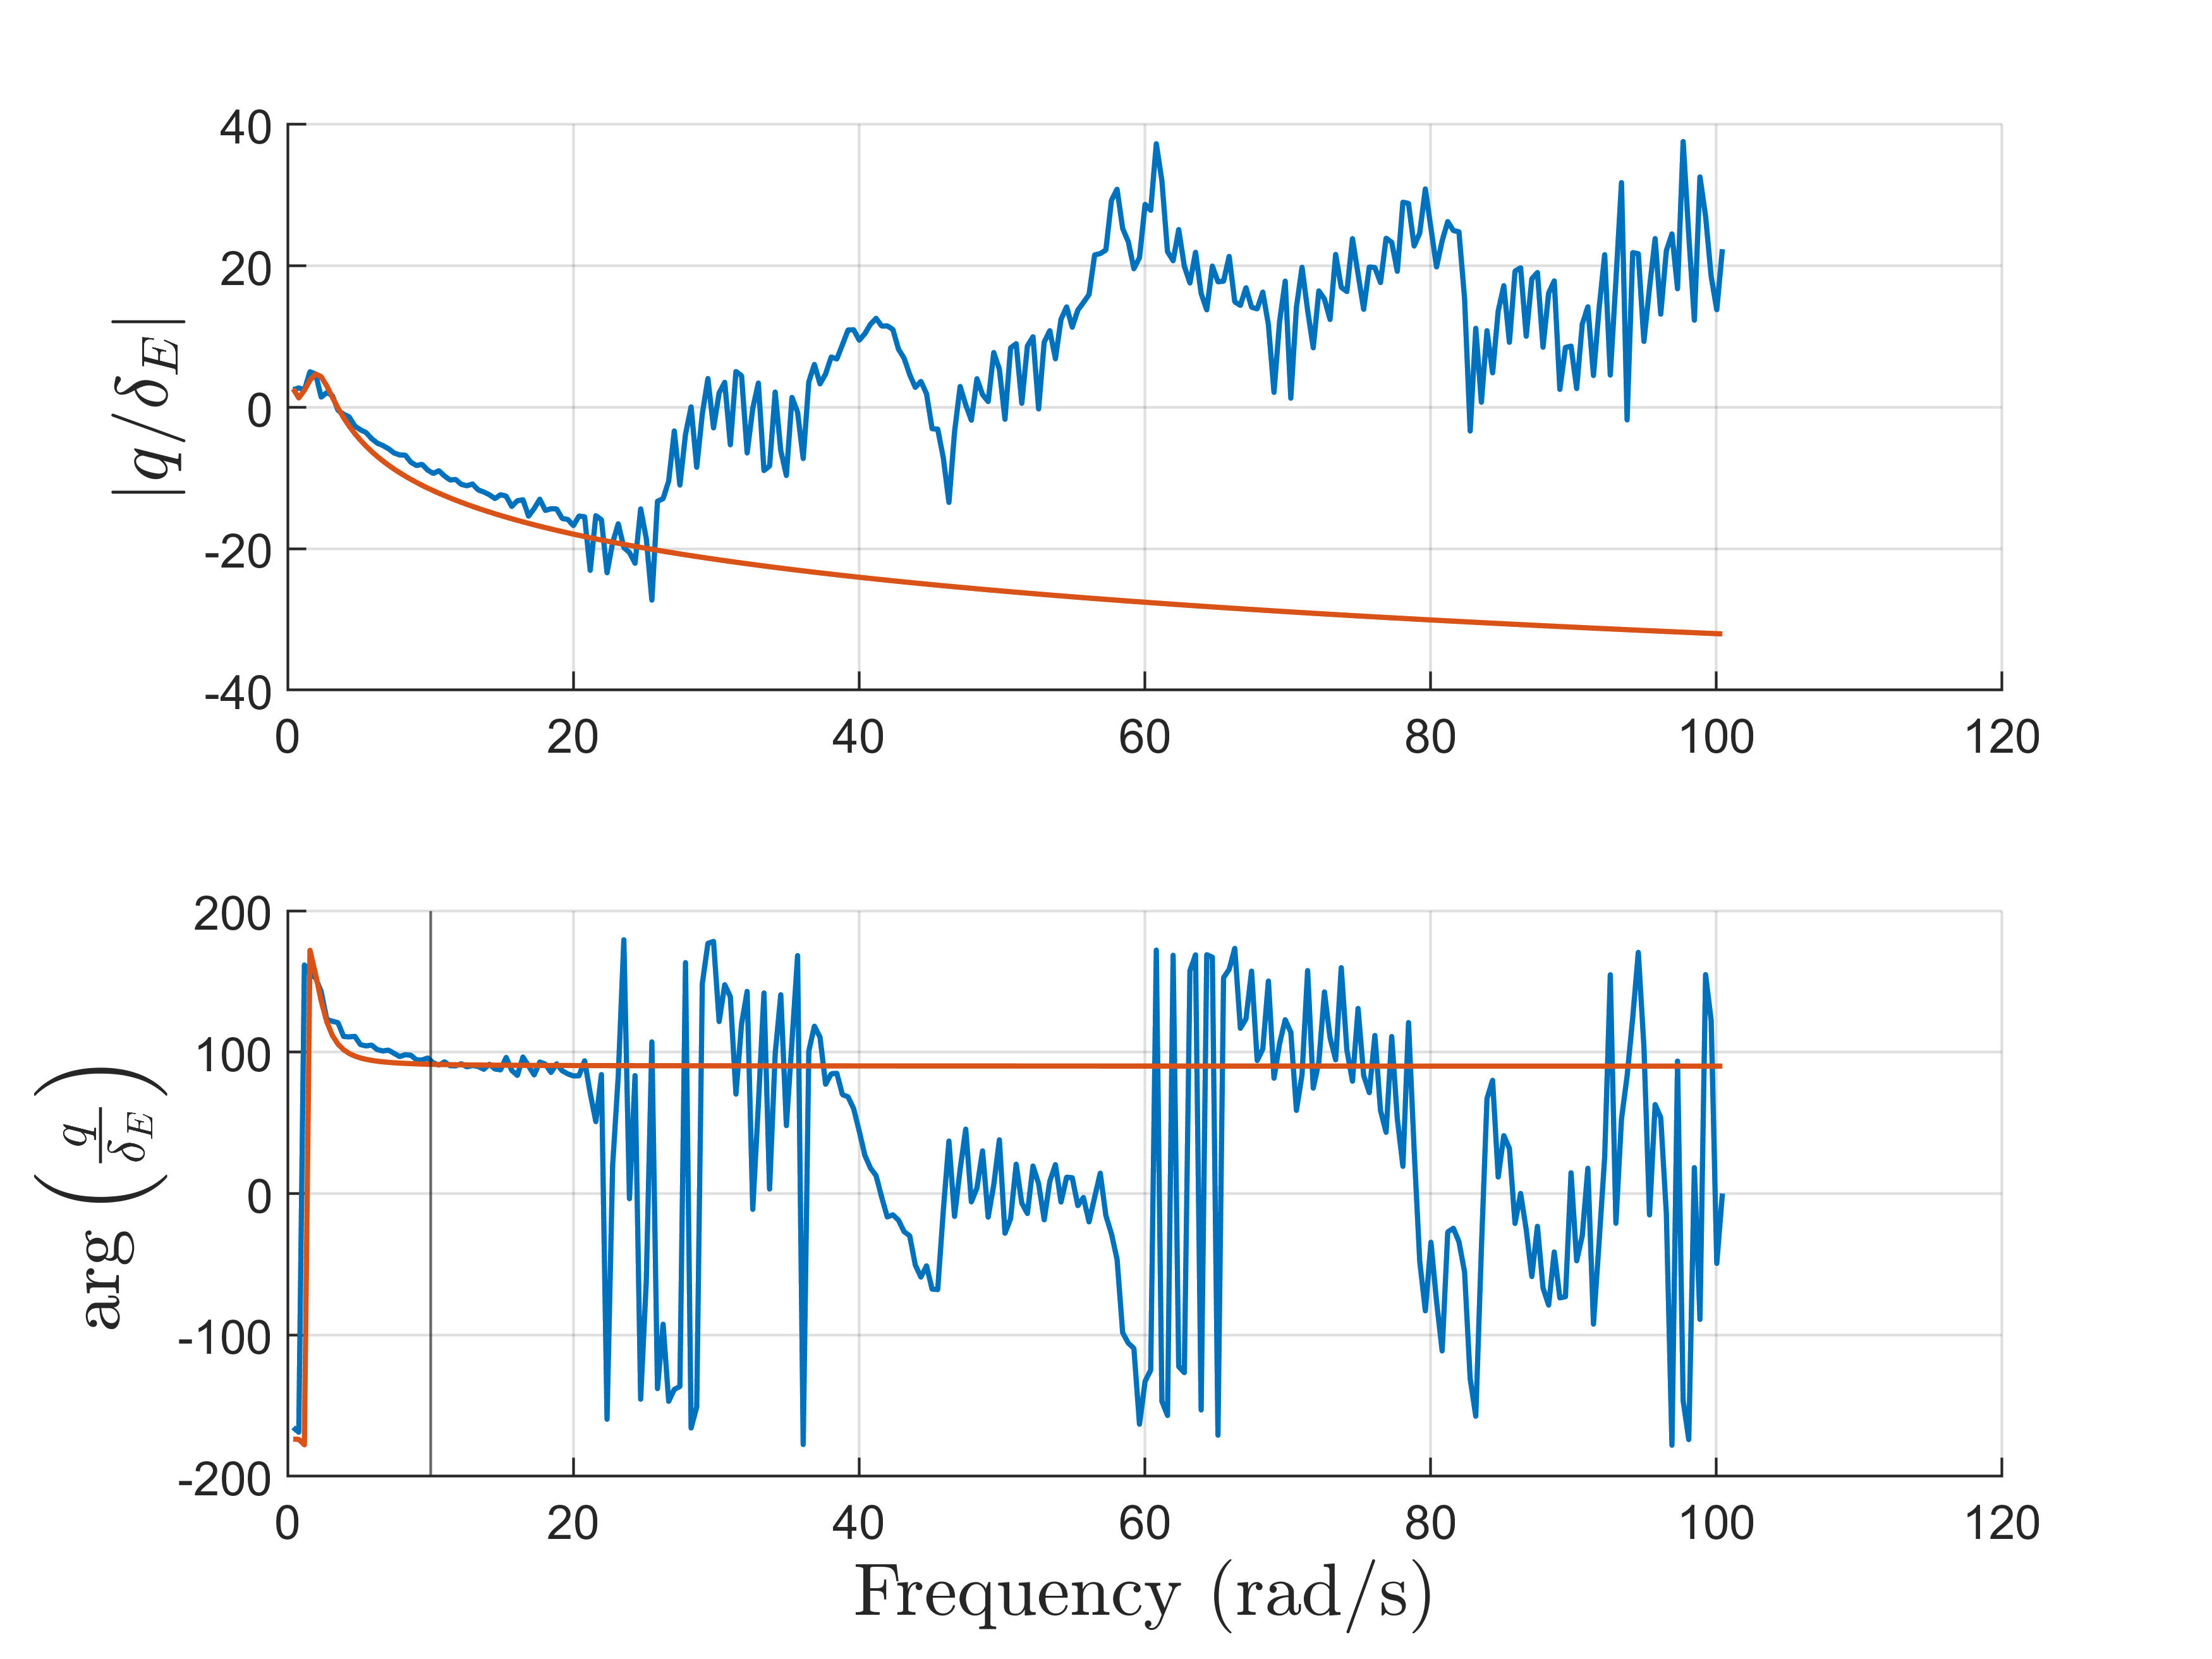
\includegraphics[width=0.6\textwidth]{elev_to_pitchrate.png}
    \caption{Transfer function from elevator angle $\delta_E$ to pitch rate $q$.}
    \label{fig:elev_to_pitchrate}
\end{figure}
  
\begin{figure}[H]
      \centering
      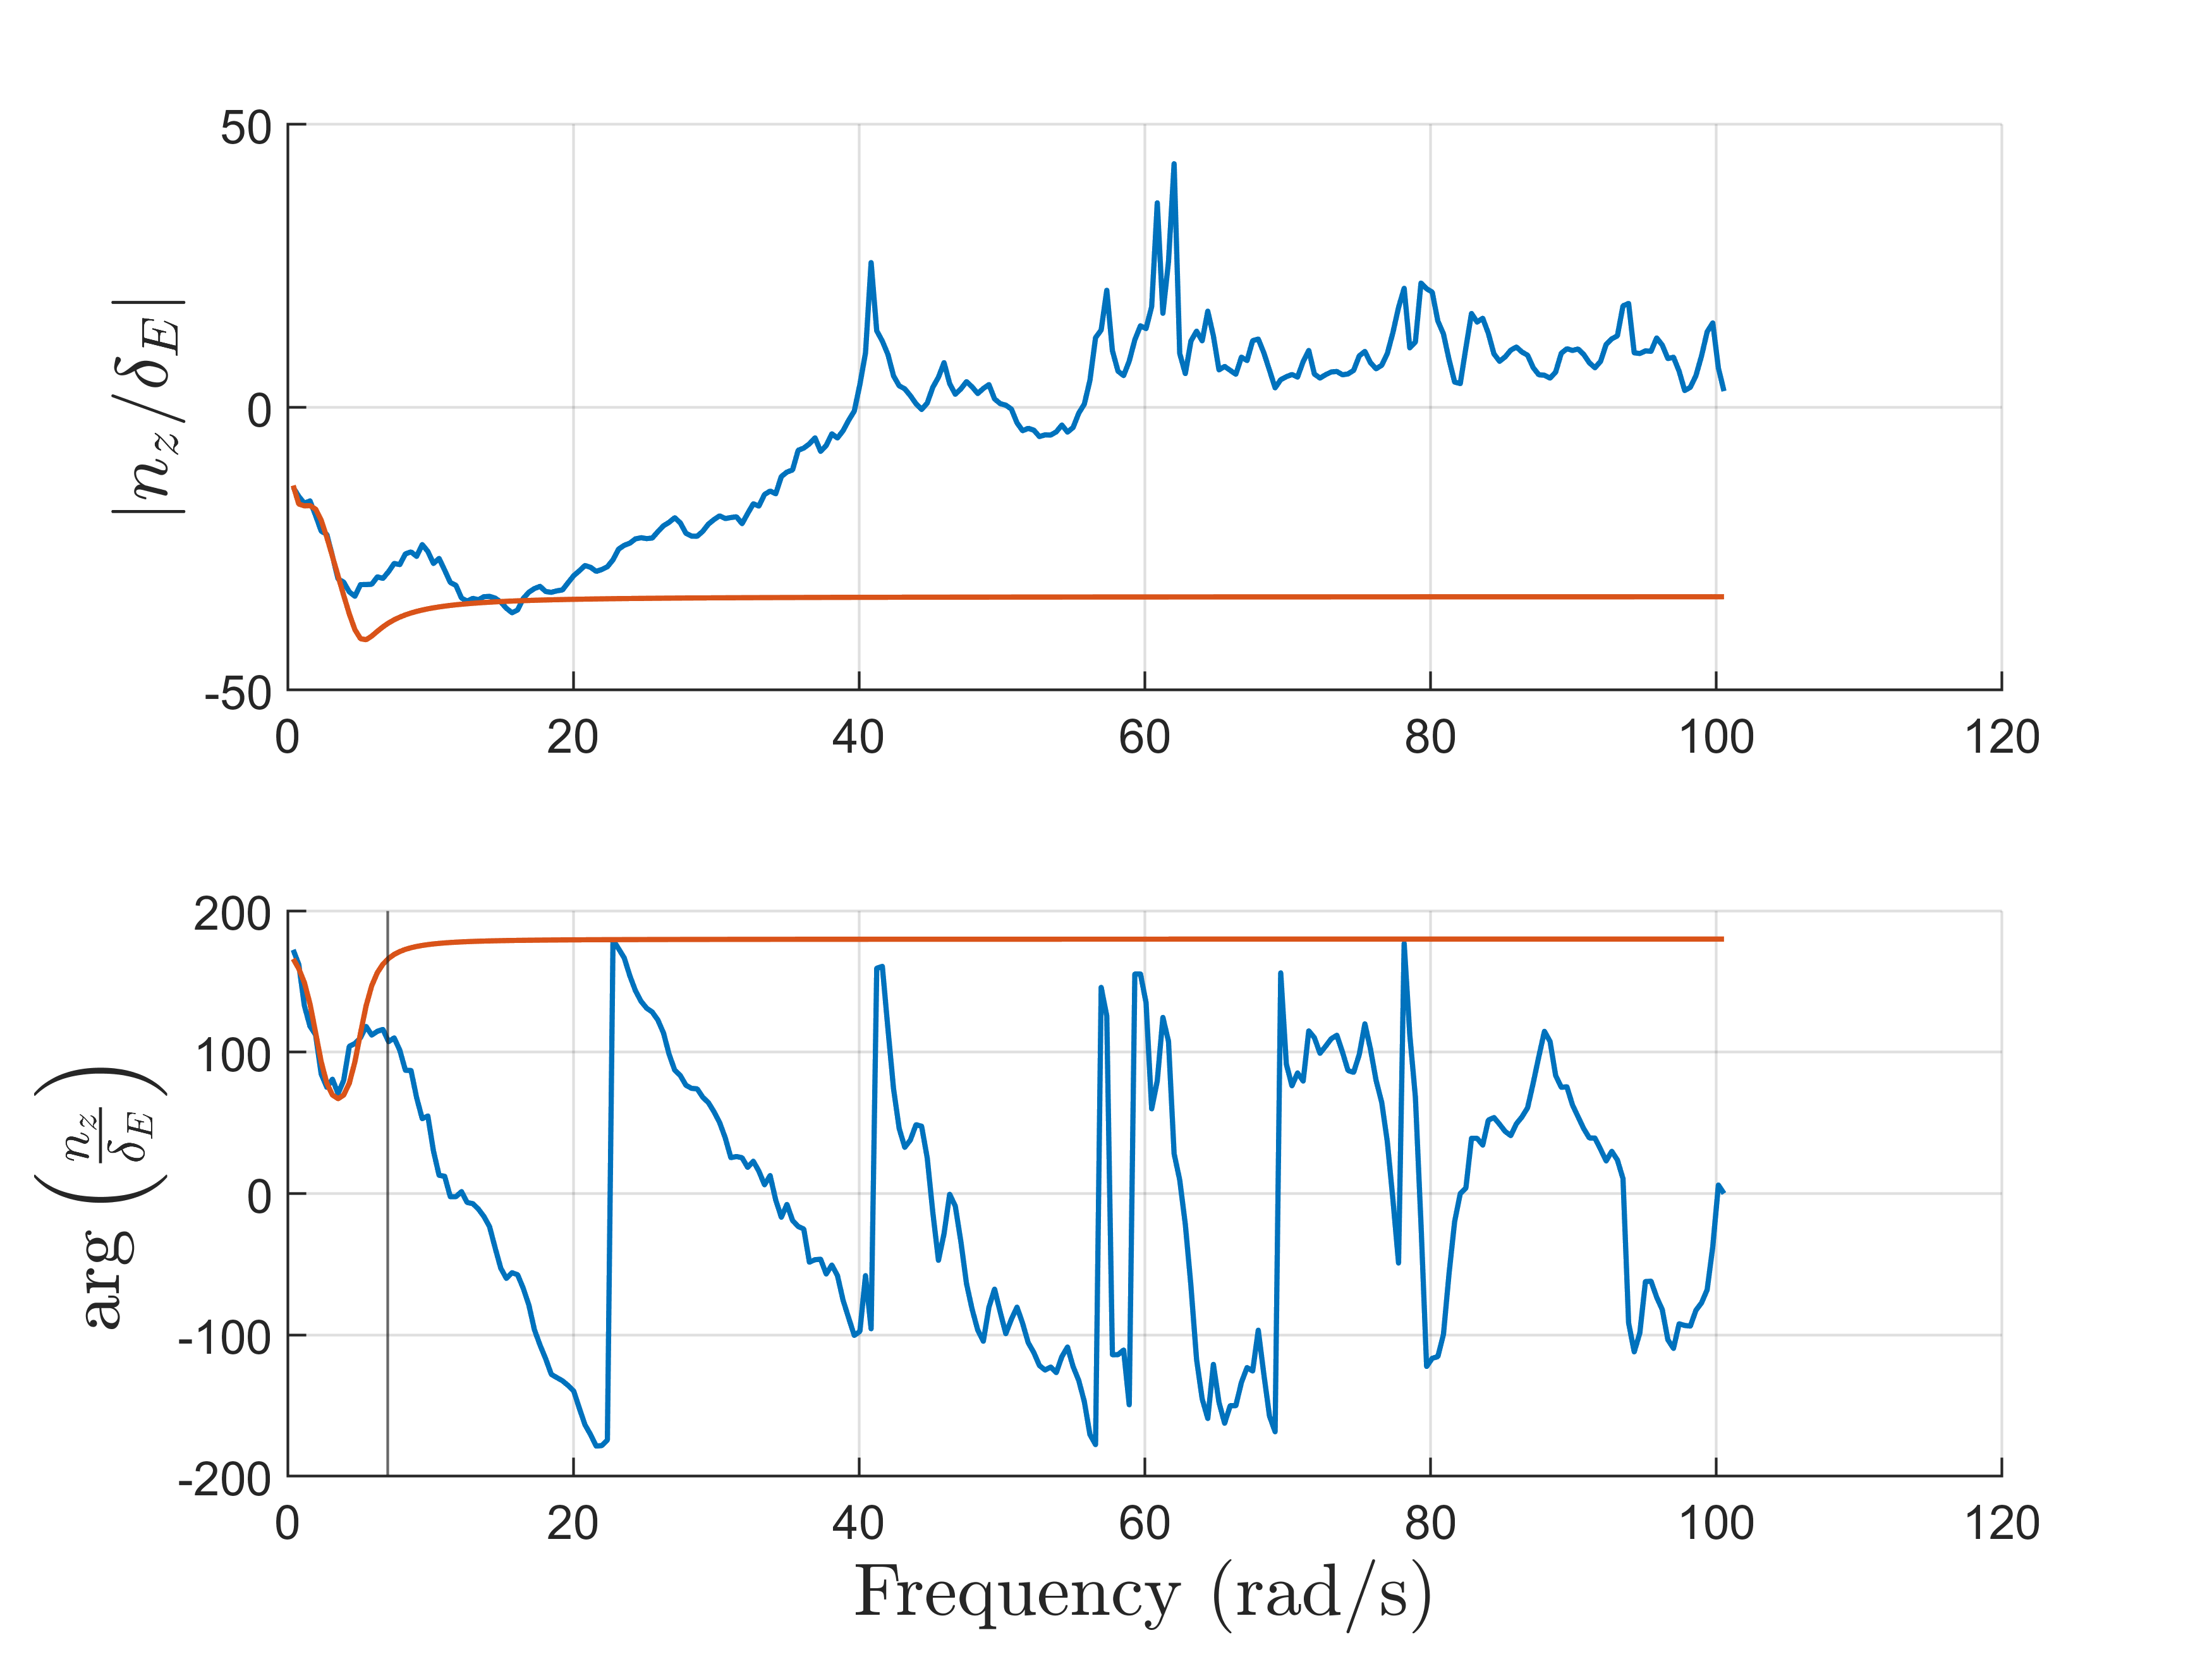
\includegraphics[width=0.6\textwidth]{elevator_to_normal.png}
      \caption{Transfer function from elevator angle $\delta_E$ to normal acceleration $n_z$.}
      \label{fig:elevator_to_normal}
\end{figure}
  
\begin{figure}[H]
      \centering
      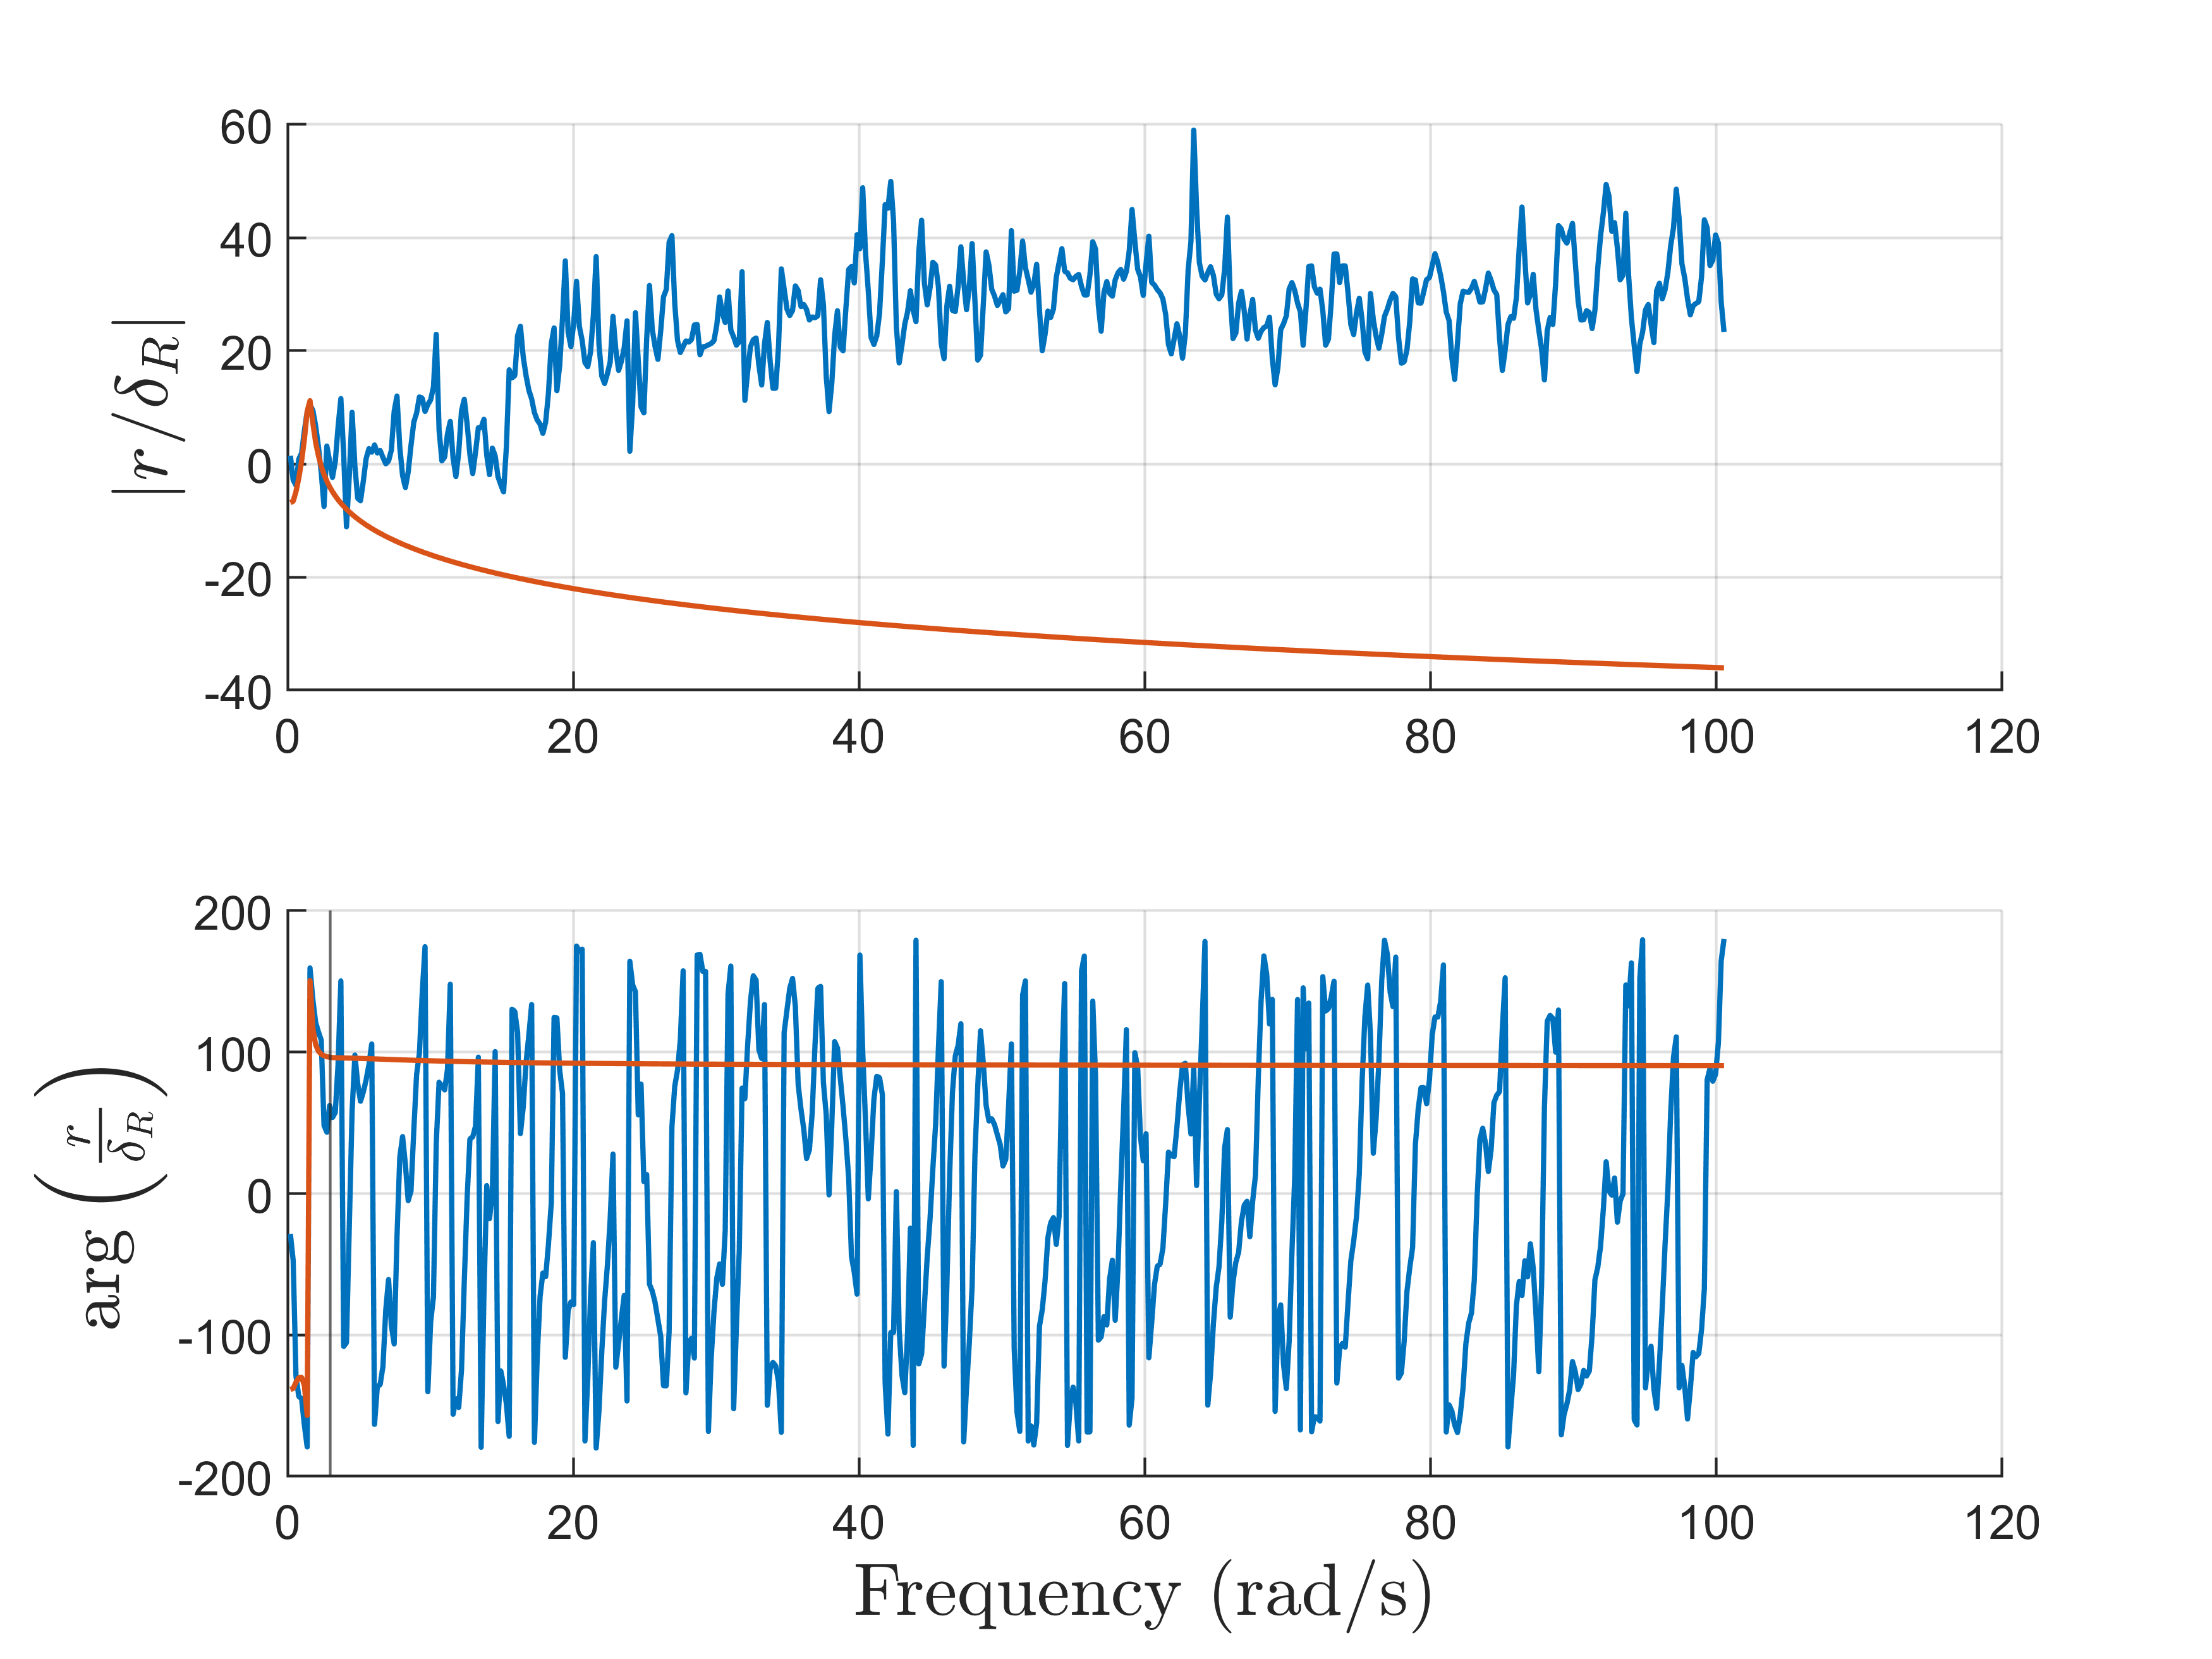
\includegraphics[width=0.6\textwidth]{rudder_to_yawrate.png}
      \caption{Transfer function from rudder angle $\delta_R$ to yaw rate $r$.}
      \label{fig:rudder_to_yawrate}
\end{figure}
  
\begin{figure}[H]
      \centering
      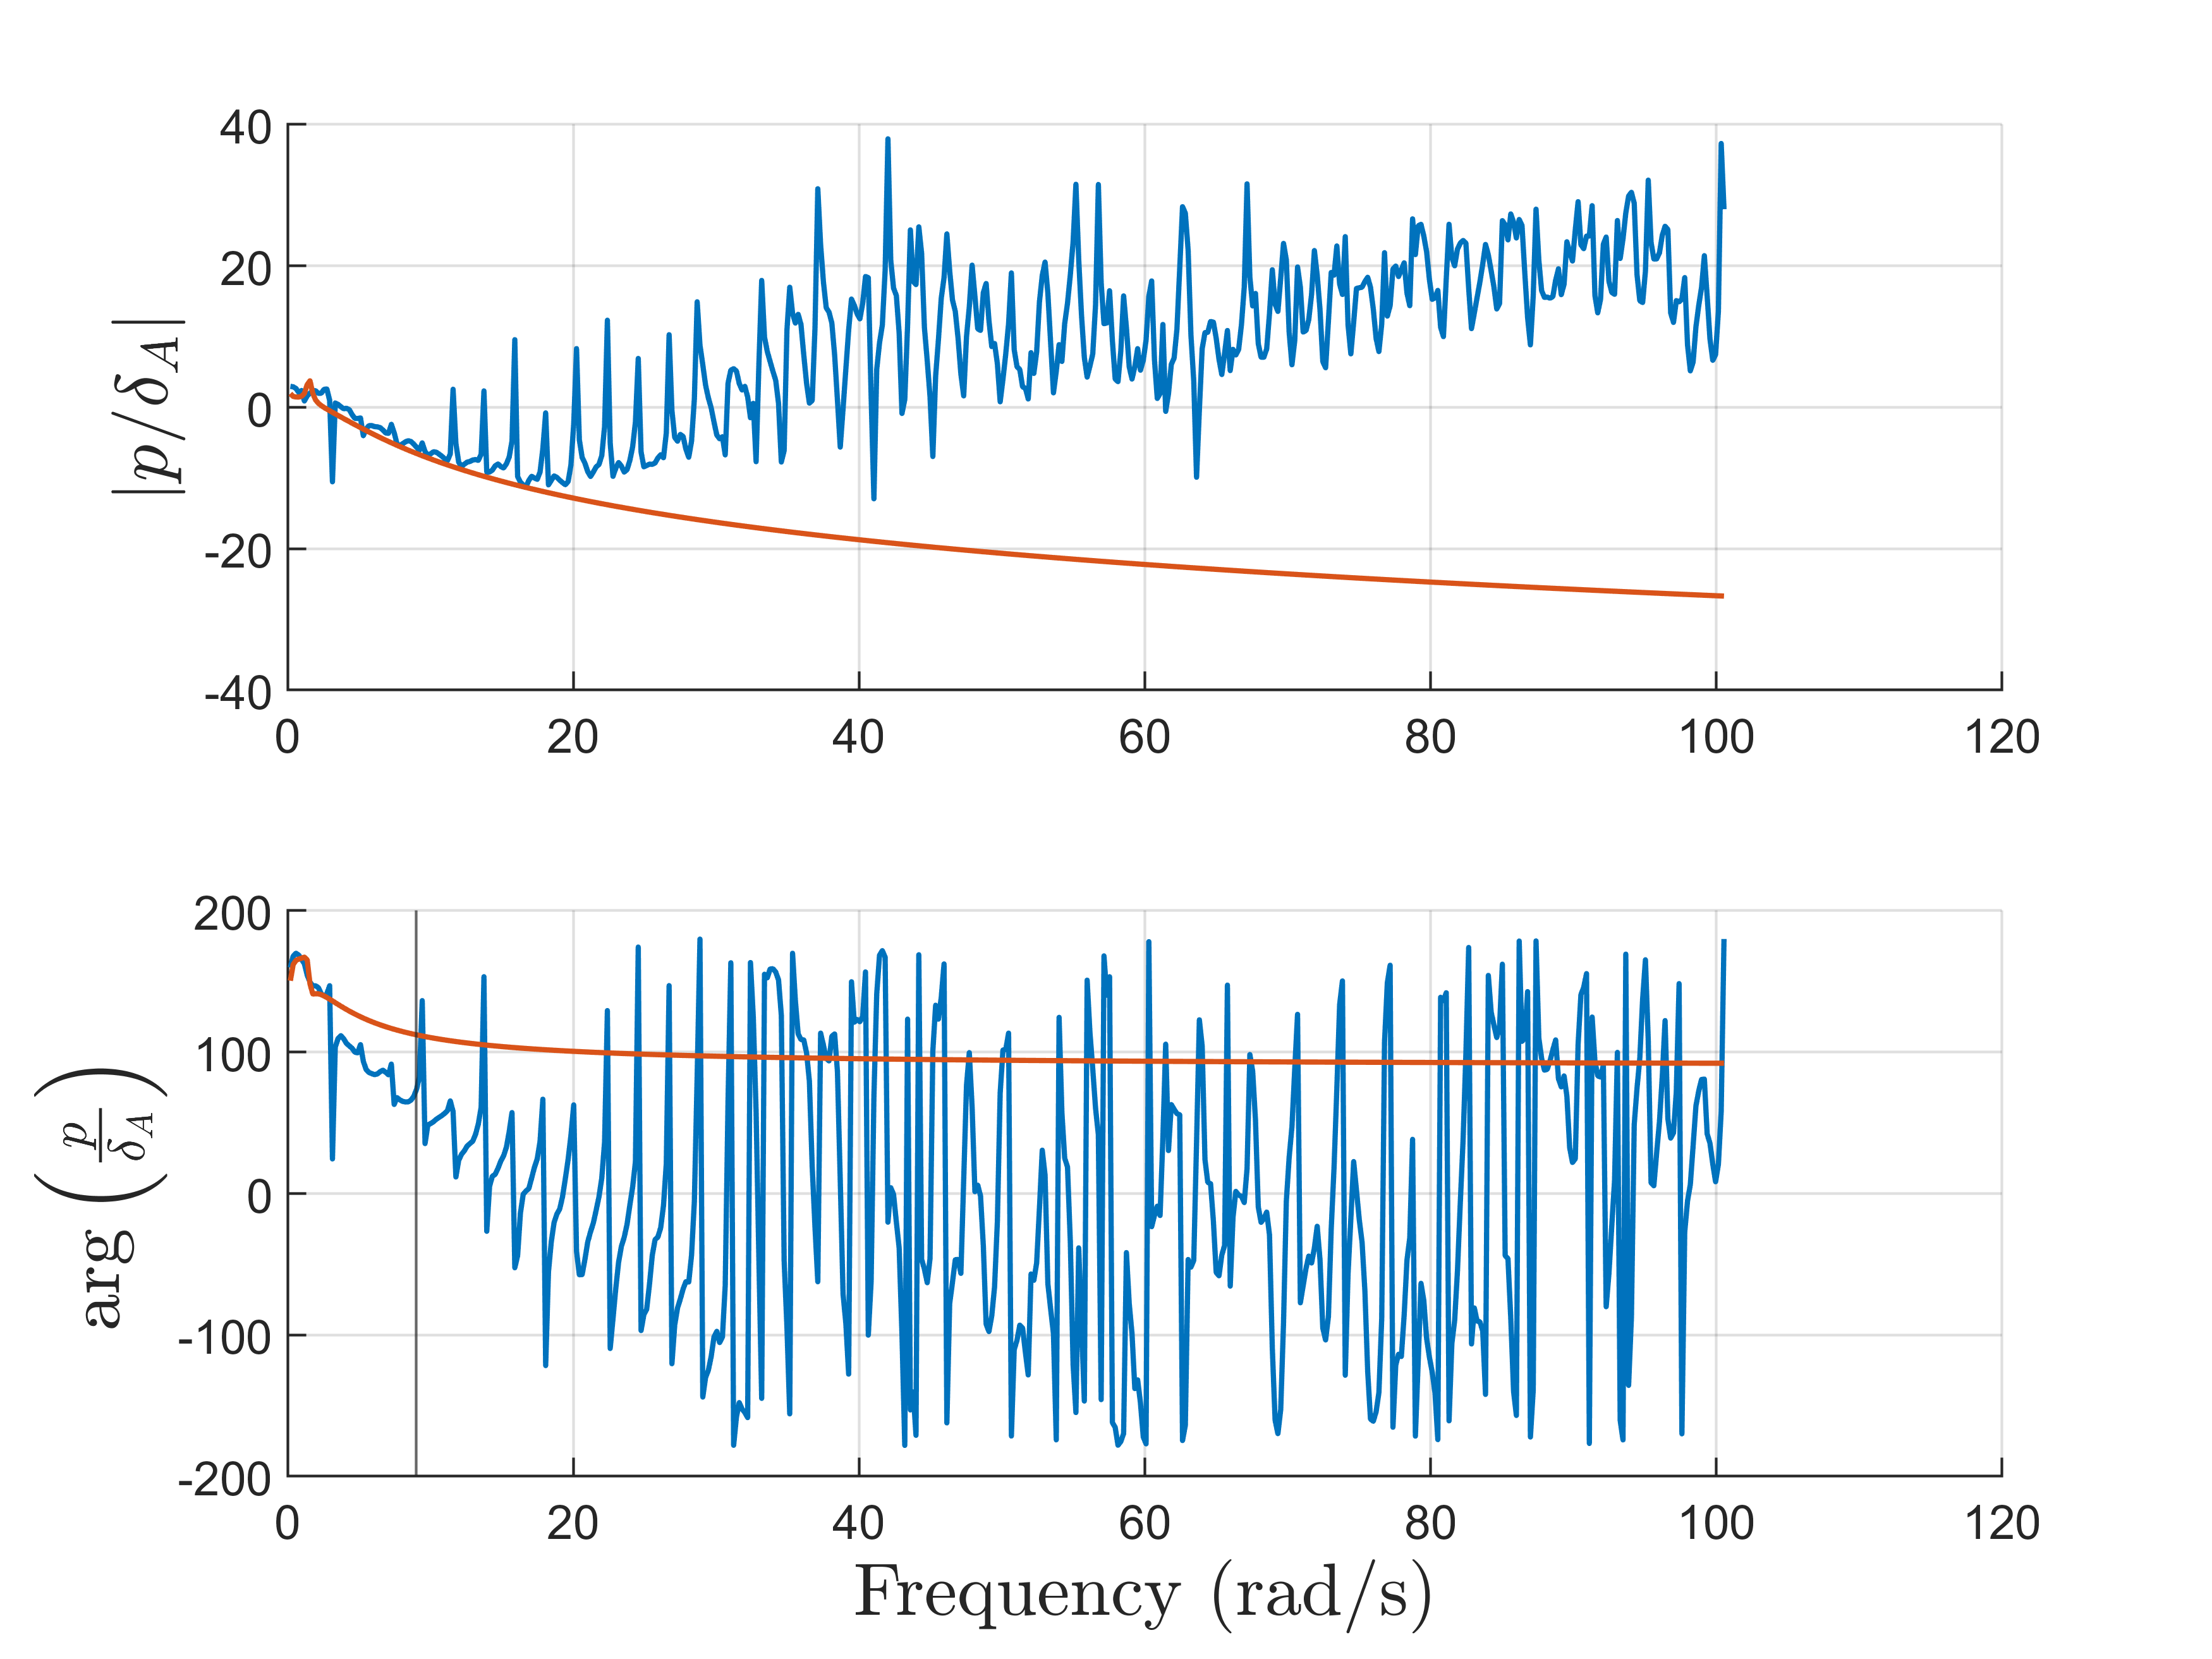
\includegraphics[width=0.6\textwidth]{aileron_to_rollrate.png}
      \caption{Transfer function from aileron angle $\delta_A$ to roll rate $p$.}
      \label{fig:aileron_to_rollrate}
\end{figure}

\section{Transfer functions}

\begin{equation}
    \frac{\theta}{\delta_E} =
    \frac{-2.50716\,s^2-4.4486\,s+0.126421}{s^4+1.92846\,s^3+5.01771\,s^2+0.105566\,s+0.0789498}
\end{equation}

\begin{equation}
    \frac{n_z}{\delta_E} =
    -\frac{0.0211993\,s^4+0.0430083\,s^3+0.556474\,s^2+0.0532744\,s-0.0509985}{s^4+1.92846\,s^3+5.01771\,s^2+0.105566\,s+0.0789498}
\end{equation}

\begin{equation}
    \frac{r}{\delta_R} =
    -\frac{1.58358\,s^3+5.6549\,s^2+2.58149\,s-0.436239}{s^4+4.34934\,s^3+3.66988\,s^2+9.17156\,s-0.217374}
\end{equation}

\begin{equation}
    \frac{\phi}{\delta_A} =
    -\frac{4.65389\,s^2+2.82347\,s^1+11.0881}{s^4+4.34934\,s^3+3.66988\,s^2+9.17156\,s-0.217374}
\end{equation}

Constant terms remaining in the fitted numerators of integrated derivatives were omitted from the above but are still significant and shown below.

For pitch angle this was found to be 0.203299, relatively large compared to the other numerator coefficients.
The roll angle had a constant term of 0.808607, which is smaller relative to the other coefficients.
This will correspond to errors in the position of zeros on the root locus plot.
The frequency range of the fit was adjusted to help reduce the values, however this proved difficult.


\section{Conclusion}

The poles were reconstructed from the modal analysis results giving denominators for longitudinal and lateral transfer functions.
Numerators were then fit to the frequency response using their known orders, and denominators.
The full transfer functions are presented.


\begin{thebibliography}{9}

  \bibitem{handout}
  S. Place, A. Cooke
  \emph{Flight Experimental Methods: Course Handbook}
  Cranfield University,

  \bibitem{e2}
  5739G
  \emph{4A4 Exercise 2: Modal Analysis of SAAB 340B Flight Data}

  \bibitem{rep}
  University of Cambridge
  \emph{Representative Mode Parameters}

\end{thebibliography}

\end{document}

